\section{FEM-Results}
Problems in \cref{cas:q_1st_Degree_Denom,cas:q_2nd_Degree_Denom,cas:q_Exponential} are solved with the following parameter values:
\begin{enumerate}	\label{itm:Parameter_Values}
	\item Each case is solved for the first three polynomial as load function:
	\begin{align*}
		f_0 \left( x \right) &= 1,	\\
		f_1 \left( x \right) &= 1 + 2x,	\\
		f_2 \left( x \right) &= 1 + 2x - 3x^2.
	\end{align*}
	\item As parameters of axial rigidity we choose
	\begin{align*}
		e_1		&= 10,	\quad e_2 = 0.01,	&& \text{in \cref{cas:q_1st_Degree_Denom,cas:q_2nd_Degree_Denom},}	\\
		\alpha	&= 1, 						&&	\text{in \cref{cas:q_Exponential}.}
	\end{align*}
	\item For the boundary conditions we set
	\begin{align*}
		\delta	&= 0,			&&		\text{in all cases,}	\\
		P 		&= 1,			&&		\text{in \cref{cas:q_1st_Degree_Denom,cas:q_2nd_Degree_Denom},}	\\
		P 		&= 0.01,		&&		\text{in \cref{cas:q_Exponential}.}
	\end{align*}
	\item Calculate each solution by both linear and cubic \glspl{basisFunction}. In each case set number of elements as
	\begin{equation*}
		N = 4, \quad N = 8, \quad  N = 16.
	\end{equation*}
\end{enumerate}
To study the solutions convergence we then compare the numerical solutions with the analytical ones
in \cref{eqn:q_1st_Degree_Denom_Solution,eqn:q_2nd_Degree_Denom_Solution,eqn:q_Exponential_Solution}.
\Cref{fig:q_1_Load_0} shows the analytical and \glspl{FEMSol} of \cref{cas:q_1st_Degree_Denom} for a uniform load,
$f_{0} \left( x \right) = 1$, as well as the parameter choices above. The three upper and lower plots visualize
\gls{linearFEMSol}s and \gls{cubicFEMSol}s, respectively.
We see clearly solution convergence of both approaches towards the \gls{analSol}, in addition to a faster one in the cubic
approach.
%
\begin{figure}
	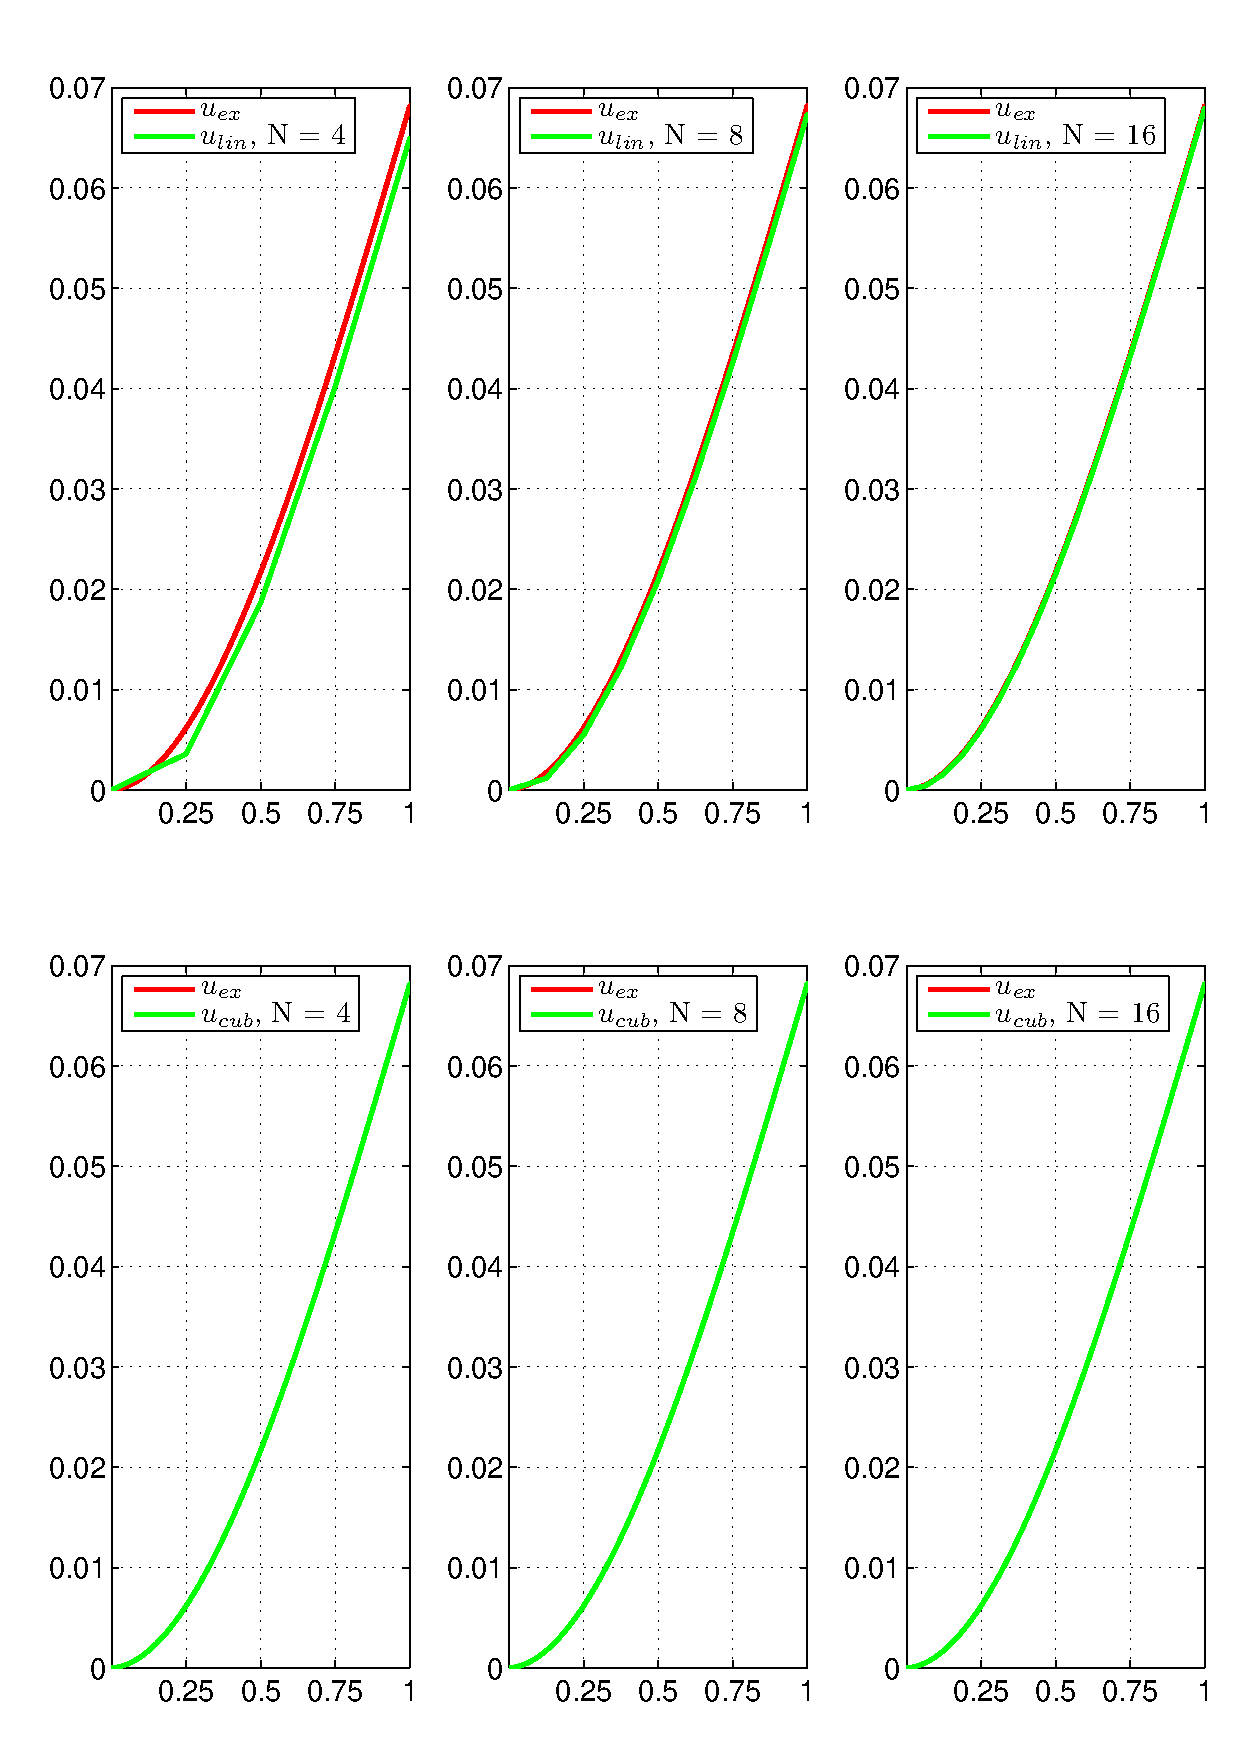
\includegraphics[width = \textwidth]{../figures/q-1-load-0}
	\caption[Analytical and \gls{FEMSol} of \cref{cas:q_1st_Degree_Denom} with a Uniform Load]
	{Analytical and \glspl{FEMSol} of \cref{cas:q_1st_Degree_Denom} with $e_1 = 10$ and $e_2 = 0.01$, a Uniform Load $\gls{f} = 1$
		and Boundary Parameters $\delta = 0$ and $P = 1$}
	\label{fig:q_1_Load_0}
\end{figure}
\begin{remark}
	As discussed in \cref{cha:Linear_Basis_Function}, \Glspl{linearFEMSol} support \glsentryname{order0Cont}. Thus
	the first derivative are discontinuous at \glspl{nodePoint}. This is clearly seen in node points when number of elements small,
	i.e., the upper left plots in \cref{fig:q_1_Load_0} The cubic solutions support, on the other hand, \glsentryname{order1Cont},
	see lower plots in the same figures.
\end{remark}
%
